\chapter{System Description}
\section{System Model}
\subsection{Overview}
Based on the scenario demonstrated in Introduction chapter, this system describes the networks that have no reliable or stable networks existed between each end-to-end entities. Entities under such conditions are regarded as off-line entities in the sense that their network is restricted and can not reach the others' networks. This system allows those off-line entities to communicate by using a Courier to deliver the message. We define 3 abstract entities in the system - Alice, Bob and Courier: we abstract all entities which originate messages as Alice, all entities who receive messages as Bob and entities who deliver messages as Courier. We assume whenever an Alice has messages to send, eventually there will be a Courier approaches her and carries messages for her. Thus, if Alice wants to send a message to Bob, the Courier firstly gets the message from Alice and stores it, then physically transports to Bob and sends the message to Bob. During the transportation, Courier has to cross a border where Courier's data will be examined by the security guard.

The goal of the system is to ensure the message from Alice to Bob is secure in the sense that no one can reveal its content but Bob. To achieve that, the Courier will never be trusted, which means the real content of the message will never be accessed by Courier and both Alice and Bob are able to deny the communication with Courier at any time. Furthermore, to prevent sensitive information from being leaked by malicious message recipient (Bob), message creator (Alice) is able to deny the message content as well.

\subsection{Initial Setting}
According to the description above, totally 3 different types of entities are defined within the system - Alice, Bob and Courier. Following specification lists the notations and jobs of those 3 entities together with the information they hold:

\begin{itemize}
\item Alice $\mathcal{A}$ denotes a set of devices who create messages and waits it to be delivered, so it is also called ``message creator". It possesses an unique ID $\mathcal{ID}_A \in \{0, 1\}^*$, a secret key $sk_A$ as part of its asymmetric key pair, and the message $\mathcal{M}$ to be sent. \\

\item Bob $\mathcal{B}$ denotes a set of devices who wait incoming messages delivered by Courier, so it is also called ``message recipient". It possesses an unique ID $\mathcal{ID}_B \in \{0, 1\}^*$, and a secret key $sk_B$ as part of its asymmetric key pair.\\

\item Courier $\mathcal{C}$ denotes a set of devices who carry the message of Alice, physically transport from Alice to Bob, and deliver the message to Bob. A single Courier will play two different roles in the system - when it receives message from Alice, it is denoted as $\mathcal{CR}$ (Courier Receiver), after that, when it delivers message to Bob, it is denoted as $\mathcal{CS}$ (Courier Sender). Initially $ \mathcal{CR} $ only possesses an unique $\mathcal{ID}_C \in \{0, 1\}^*$. After it gets messages from Alice and before it delivers message to Bob, it plays as $\mathcal{CS}$ and possesses some more information: the ID of message recipient $ \mathcal{ID}_B $ and the encrypted message received from $\mathcal{A}$.
\end{itemize}

\paragraph{Public Key Distribution}
The distribution of asymmetric key pairs used for authentication is out of the scope of this system, thus $\mathcal{A}$ and $\mathcal{B}$ are assumed to hold their asymmetric key pairs before the communication. Furthermore, all entities in the system are assumed to know each other's public key (does not matter it is distributed with manufacture, authenticated by CA, or by key exchange), before the communication.

\paragraph{Devices v.s. Entities}
A device $x$ denotes a physical object within the system. Differently, an entity denotes a particular role in the system. It should be noted that any device can communicate with multiple other devices simultaneously, thus a single device can be any both $ \mathcal{A} $ and $ \mathcal{B} $ at the same time. The role it plays in different communications is defined by what information $x$ holds and what its behaviour is (detail will be described in Trusted Entity Behaviour). On the contrary, an entity in the system can be associated with only one device.

\subsection{Communication Model}
Within the system, there will be several message creators $ \mathcal{A} $ and they possibly will send messages to different message recipients $ \mathcal{B} $ simultaneously, thus a single courier is able to collect messages from multiple message creators at a time. Because the storage capability of single courier is limited, to keep the fairness between each message creator, each message creator can submit maximumly one message to a courier at a time. Typically, a single communication requires courier collects all data from message creators and transports them to all message recipients. However, because each communication between several message creators and a single message recipient is totally independent with each other, the whole communication can be regarded as several independent M-to-1 communications. For example, achieving communication of $a_0 \in \mathcal{A}$ sends message to $ b_0 \in \mathcal{B} $ and $a_1 \in \mathcal{A}$ sends message to $ b_1 \in \mathcal{B} $ using a single courier can be regarded as achieving two independent communications which are (1) $a_0 \in \mathcal{A}$ sends message to $ b_0 \in \mathcal{B} $, and (2) $a_1 \in \mathcal{A}$ sends message to $ b_1 \in \mathcal{B} $ using two couriers, from the view of the system, they are totally the same. To simplify the communication model, it will be discussed under a M-to-1 model - M message creators each send one message to a single message recipient, as it is the primary model.

An abstract M-to-1 communication involves following entities: a certain number of off-line devices $a_0, a_1, ... a_M \in \mathcal{A}$ send messages to a single off-line device $b \in \mathcal{B}$ independently, using a device $c \in \mathcal{C}$ as media. As physical transportation is slow and costly, the total number of physical transportation is expected to reduce to minimum. The optimized solution appeared to be separating the communication into two main phases - Message Acquisition phase and Message Delivery phase. In Message Acquisition phase, the courier $c$ will physically transport to every $a \in \mathcal{A}$ one by one, connect to it and get the message that is for $b$. After $c$ collects all needed messages, it enters Message Delivery phase, where $c$ transports to $b$ and transmit all acquired messages to it.

According to explanation above, the whole task can be divided into M + 1 individual sub-communications. In Message Acquisition phase, the courier establishes a sub-communication with each $a$ to get message from it, and in Message Delivery phase, the courier establishes sub-communication with $b$ to transmit messages to it. All these sub-communications are assumed to be established by typical network communication methods (e.g. cable, Wifi, Bluetooth, etc.) and apply their corresponding communication protocols (e.g. TCP/IP, UDP, Bluetooth protocol, etc.). The following figure shows how the communication is organized.

\begin{figure}[h!]
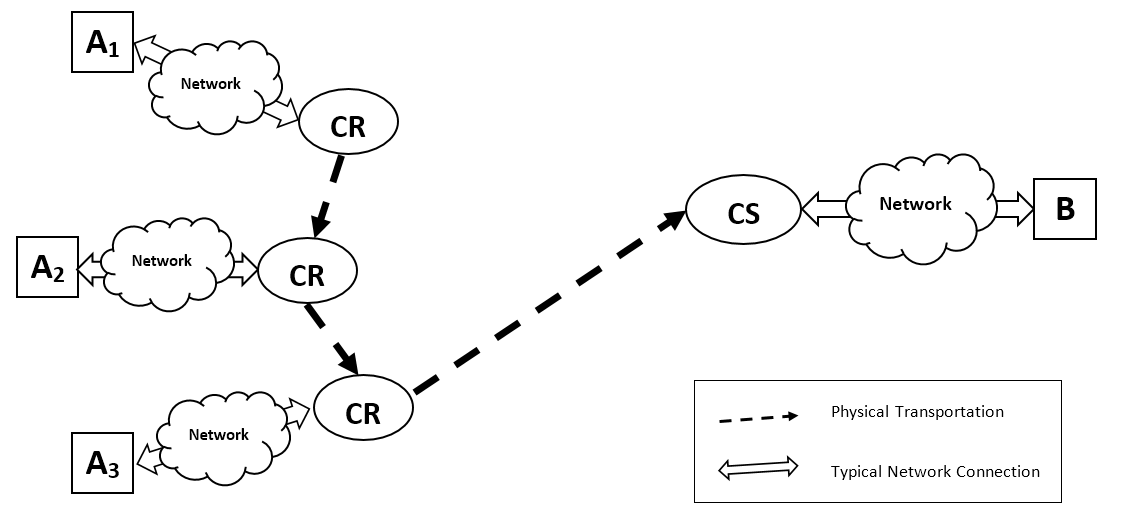
\includegraphics[width=\textwidth,natwidth=1123,natheight=530]{figures/communicationmodel.png}
\caption{Communication Model}
\end{figure}

The figure "Communication Model" illustrates the procedure of a 3-to-1 communication. The Courier first connects to A$_1$, be the role of $\mathcal{CR}$, and gets A$_1$'s message for B through the connection, then disconnects and transports to A$_2$. It should do the same thing to A$_2$ and then transport to A$_3$. After it collects all data from A$_1$, A$_2$ and A$_3$, it transports to B and be the role of $\mathcal{CS}$ to send all collected messages to B. The networks between Courier and As or B can use any kind of typical network communication methods and do not have to be same, as long as both entities agree. 

\subsection{Honest Entity Behaviour}
To achieve the communication, all three entities $ \mathcal{A} $, $ \mathcal{B} $, $ \mathcal{C} $ have different behaviour patterns, the actions they can take to interact with the rest of the system are listed respectively in the following description:

\paragraph{Alice $\mathcal{A}$}
\begin{itemize}
\item If Alice wants to send a message, it takes a timestamp when creating the message. Then it continuously listening to its network, waiting for incoming Couriers.

\item Once a Courier connects to Alice, Alice immediately submits its message the Courier and explicitly specifies a message recipient.

\item When Alice is submitting a message, she can stop the submitting process at any time.

\item After Alice submits a message to a Courier, she can deny sending the message to the Courier at any time.

\item If the message is not successfully sent, Alice waits for next Courier to send this message.

\item Alice is allowed to submit any message arbitrary times, to as many Couriers as she wants. Alice herself does not care who carries her messages, nor how many Couriers carry her message.
\end{itemize}

\paragraph{Bob $\mathcal{B}$}
\begin{itemize}
\item Bob must be continuously listening to its network, waiting for incoming Couriers.

\item Once a Courier connects to Bob, Bob downloads all messages from the Courier. Then Bob checks the messages received. If any message is invalid, Bob simply discards it.

\item Bob will discard all duplicated messages. Duplicated message are defined as messages whose creator IDs and timestamps are exactly the same. Because timestamp is created at the time that the message is created, sharing same IDs and timestamps reflects those messages are created by the same entity at the exact same time.

\item When Bob is downloading a message, he can stop the downloading process at any time.

\item After Bob receives a message from a Courier, he can deny receiving the message from the Courier at any time.
\end{itemize}

\paragraph{Courier $\mathcal{C}$}
\begin{itemize}
\item As Courier's physical transportation is a very complicated task, it is out of the scope of this protocol. It is assumed that Courier is controlled by an intelligent agent (such like human) who always knows where other entities located.

\item Courier chooses some of the potential message creators to deliver messages for them. The specific choosing process is not defined in the system model. It can be regarded as (1) Courier routinely check all devices in the system, see if they have messages to send, or (2) The intelligent agent who controlled the Courier ``magically" knows which device has message to send.

\item Courier transports to every chosen message creators one by one and get their messages if they have.

\item After collect messages from all chosen message creators, it crosses the border and transports to every message recipients that are specified by those message creators.

\item Once Courier transports to a message recipient, it transmits all corresponding messages (which is designated to be delivered to this recipient) to it.

\item If any transmission failed, Courier tries to retransmit, until it succeeds or Courier decides to abandon the transmission.

\item Once a message has been successfully transmitted to its recipient, it is erased from the storage of Courier and will not make any effects in future.
\end{itemize}

\section{Adversary Model}
\subsection{Adversary Capability}
The adversary model in this system is mostly derived from Dolev-Yao model which implies ``adversary carries the message" in the network \cite{Dolev}. Moreover, the adversary can also do something particular in this system. Specifically, an adversary $ \mathcal{Z} $ has following capabilities:
\begin{itemize}
\item It supervises the whole network system, which means it knows when, where and how  entities are communicating, and it knows what information is held by each entity in the system.
\item It can access/rewrite any message passing through the network.
\item It is a legitimate user of the system.
\item It can access to all the Courier's data at any time.
\item It will always have opportunity to be contacted by any other honest entities.
\end{itemize}

\subsection{Adversary Goal}
The goal of the adversary $ \mathcal{Z} $ is various, it depends on what role it plays in a certain communication.
\begin{itemize}
\item If $ \mathcal{Z} $ is \textbf{not involved} in a particular communication, its goal is to:
 \begin{enumerate}
 \item reveal the message content exchanged in the communication
 \item modify the message sent by message creator and make it accepted by the message recipient
 \item impersonate the message creator or message recipient
 \item prove the identities of message creator and message recipient to any third parties.
 \end{enumerate}

\item If $ \mathcal{Z} $ acts as \textbf{courier} in a communication, its goal is to:
 \begin{enumerate}
 \item reveal the message content exchanged in the communication
 \item modify the message sent by message creator and make it accepted by the message recipient
 \item prove the identities of the message creator and message recipient to third parties
 \item forge a message and make it accepted by any message recipient
 \end{enumerate}
 
\item If $ \mathcal{Z} $ acts as \textbf{message recipient} in a communication, its goal is to prove the authenticity of the message content to any third parties.
\end{itemize}

It should be noted that this network system is vulnerable to DoS attacks - same as any other existing network systems. It means $\mathcal{Z}$ can always prevent a message from being successfully delivered. However, it is not listed in the adversary goal, thus it will not be covered in the system security analysis.